\chapter{Overview of Eigenvalue Algorithms}
This and the next five chapters describe some of the classical ``direct'' algorithms for computing eigenvalues and eigenvectors, as well as a few modern variants. Most of these algorithms proceed in two phases: first, a preliminary reduction from full to structured form; them , an iterative process for the final convergence. This lecture outlines the two-phase approach and explains why it is advantageous. 

\section{Shortcomings of Obvious Algorithms}
Perhaps the first method one might think of would be to compute the coefficients of the characteristic polynomial and use a rootfinder to extract its roots. UNfortunately, as mentioned in Chapter 14, this strategy is a bad one, because polynomial rootfinding is an ill-conditioned problem in general, even when the underlying eigenvalue problem is well-conditioned. (In fact, polynomial rootfinding is by no means a mainstream topic in scientific computing -- precisely because it is so rarely the best way to solve applied problems.)  

Another idea would be to take advantage of the fact that the sequence
\[
\frac{x}{\|x\|}, \frac{Ax}{\|Ax\|}, \frac{A^2x}{\|A^2x\|}, \frac{A^3x}{\|A^3x\|},\ldots  
\] 
converges, under certain assumptions, to an eigenvector corresponding to the largest eigenvalue of $A$ in absolute value. THis method for finding an eigenvector is called \textbf{power iteration}. Unfortunately, although power iteration is famous, it is by no means an effective tool for general use. Except for special matrices, it is very slow.  

Instead of ideas like these, the best general purpose eigenvalue algorithms are based on a different principle: the computation of an eigenvalue-revealing factorization of $A$, where the eigenvalues appear as entries of one of the factors. We saw three eigenvalue-revealing factorizations in the last lecture: diagonalization, unitary diagonalization, and unitary triangularization (Schur factorization). In practice, eigenvalues are usually computed by constructing one of these factorizations. Conceptually, what must be done to achieve this is to apply a sequence of transformations to $A$ to introduce zeros in the necessary places, just as in the algorithms we have considered in the preceding chapters. Thus we see that finding eigenvaleus ends up rather similar in flavor to solving systems of equations or least square problems. The algorithms of numerical linear algebra are mainly built upon one technique used over and over again: putting zeros into matrices. 

\section{A Fundamental Difficulty} 
Though the flavors are related, however, a new spice appears in the dish when it comes to computing eigenvalues. What is new is that it would appear that algebraic considerations must preclude the success of any algorithm of this kind. 

To see the difficulty, note that just as eigenvalue problems can be reduced to polynomial rootfinding problems, conversely, any polynomial rootfinding problem can be stated as an eigenvalue problem. Suppose we have the monic polynomial 
\[
    p(z) = z^m + a_{m-1}z^{m-1} + \cdots + a_1z + a_0. 
\]
It's not hard to verify that $p(z)$ is equal the determinant of the $m\times m$ matrix 
\[
    \begin{bmatrix}[] 
        -z &  &  &  &  &  -a_0 \\
        1 & -z &  &  &  &  -a_1 \\
         & 1 & -z &  &  &  -a_2 \\
         &  & 1 & \ddots &  &  \vdots \\
         &  &  & \ddots & -z &  -a_{m-2} \\
         &  &  &  & 1 &  (-z-a_{m-1}) \\
    \end{bmatrix} . 
\]
This means that the roots of $p$ are equal to the eigenvalues of the matrix 
\[
    A = \begin{bmatrix}[] 
        0 &  &  &  &  &  -a_0 \\
        1 & 0 &  &  &  &  -a_1 \\
         & 1 & 0 &  &  &  -a_2 \\
         &  & 1 & \ddots &  &  \vdots \\
         &  &  & \ddots & 0 &  -a_{m-2} \\
         &  &  &  & 1 &  -a_{m-1} \\
    \end{bmatrix} . 
\]
     
Here $A$ is called a \textbf{companion matrix} corresponding to $p$.  Now the difficulty is apparent. It's well known that no formula exists for expressing the roots of an arbitrary polynomial, given its coefficients. Abel proved in 1824 that no analogue of the quadratic formula can exist for polynomials of degree 5 or more.  

This does not mean that we cannot write a good eigenvalue solver. It does mean, however, that such a solver cannot be based on the same kind of techniques that we have used so far for solving linear systems. Methods like Householder reflections and Gaussian elimination would solve linear systems of equations exactly in a finite number of steps if they could be implemented in exact arithmetic. By contrast, 
\[
    \text{ Any eigenvalue solver must be iterative. }
\]
The goal of an eigenvalue solver is to produce sequences of numbers that converge rapidly towards eigenvalues. In this respect eigenvalue computations are more representative of scientific computing than solutions of linear systems of equations.  

\section{Schur Factorization and Diagonalization} 
Most of the general purpose eigenvalue algorithms in use today proceed by computing the Schur factorization. We compute a Schur factorization $A= Q TQ^*$ by transforming $A$ by a sequence of elementary unitary similarity transformations $X \mapsto Q_j^* XQ_j$, so that the product 
\begin{equation}
\label{eq: schur form}
Q_j^*\cdots Q_2^* Q_1^*  A Q_1 Q_2 \cdots Q_j    
\end{equation}
converges to an upper-triangular matrix $T$ as $j\to \infty$. 

If $A$ is real but not symmetric, then in general it may have complex eigenvalues in conjugate pairs, in which case its Schur form will be complex. Thus an algorithm that computes the Schur factorization will have to capable of generating complex outputs from real inputs.  This can certainly be done. Alternatively, it's possible to carry out the entire computation in real arithmetic if one computes what is know as a areal Schur factorization. Here, $T$ is permitted to have $2\times 2$ blocks along the diagonal, one for each complex conjugate pair of eigenvalues. This option is important in practice, and is included in all the software libraries.  

\section{Two Phases of Eigenvalue Computations} 
Whether or not $A$ is hermitian, the sequence \eqref{eq: schur form} is usually split into two phases. In the first phase, a direct method is applied to produce an upper-Hessenberg matrix $H$, that is, a matrix with zeros below the first subdiagonal. In the second phase, an iteration is applied to generate a formally infinite sequence of Hessenberg matrices that converge to a triangular form. Schematically, the process looks like this: 
%────────────────────────────────────────
\begin{figure}[H]
    \centering
    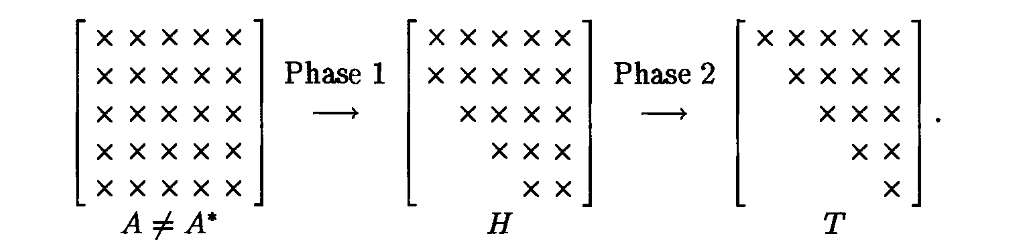
\includegraphics[width=0.8\textwidth]{figures/25-1.png}
\end{figure}
%────────────────────────────────────────
The first phase, a direct reduction, requires $O(m^3)$ flops. The second, iterative phase never terminates in principle, and if left to run forever would require an infinite number of flops. However, in practice, convergence to machine precision is achieved in $O(m)$ iterations. Each iteration requires $O(m^2)$ flops, and thus the total work requirement of $O(m^3)$ flops. These figures explain the importance of Phase 1. Without that preliminary step, each iteration of Phase 2 would involve a full matrix, requiring $O(m^3)$ work, and this would bring the total to $O(m^4)$-- or higher, since convergence might also sometimes require more than $O(m)$ iterations.  

If $A$ is hermitian, the two-phase approach becomes even faster. The intermediate matrix is now a hermitian Hessenberg matrix, that is, \textbf{tridiagonal}. The final result is a hermitian triangular matrix, that is, diagonal, as mentioned above. Schematically: 
%────────────────────────────────────────
\begin{figure}[H]
    \centering
    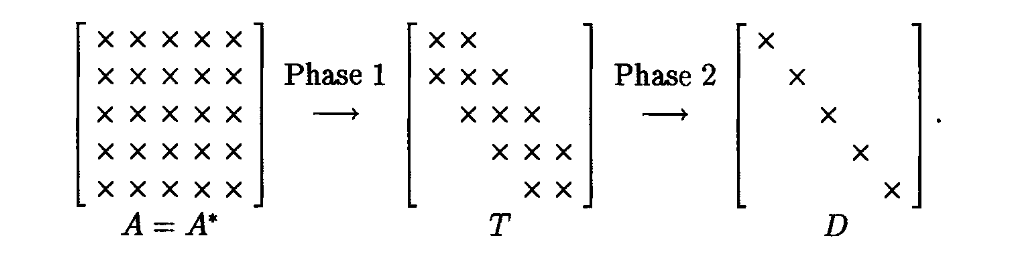
\includegraphics[width=0.8\textwidth]{figures/25-2.png}
\end{figure}
%────────────────────────────────────────
In this hermitian case, we shall see that if only eigenvalues are required, then each step of Phase 2 can be carried out with only $O(m)$ flops. Bringing the total work estimate for Phase 2 to $O(m^2)$ flops. Thus, for hermitian eigenvalue problems, we are in the paradoxical situation that the ``infinite'' part of the algorithm is in practice not merely as fast as the ``finite'' part, but an order of magnitude faster.  

